\section{Dataset}
\label{sec:dataset}
\begin{figure}[t]
	\begin{center}
		
\includegraphics[width=0.4\textwidth]{Matt_LeBlanc_as_Joey_Tribbiani.jpg}
	\end{center}
	\caption{Joey from Friends televisions show. Played by Matt LeBlanc. Image download from Wikipedia and originally from Friends' press release.}
	\label{fig:friends_data_extracted}
\end{figure}
\begin{figure}[t]
	\begin{center}
		\fbox{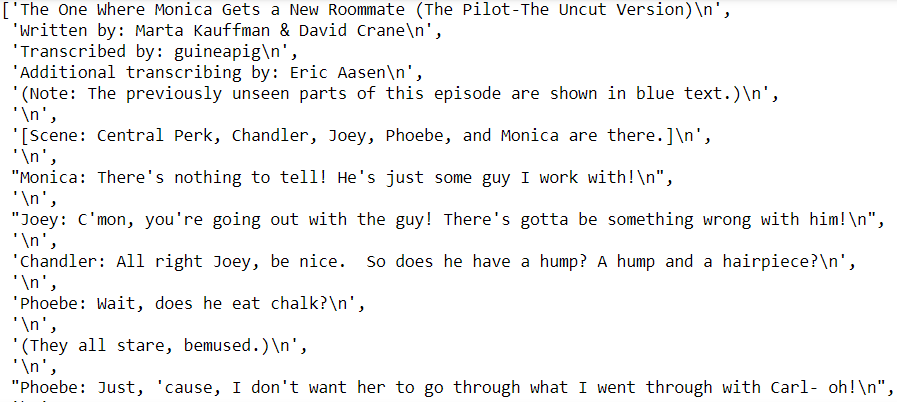
\includegraphics[width=\textwidth]{rawData.PNG}}
	\end{center}
	\caption{Example script content from Friends dataset.}
	\label{fig:friends_data}
\end{figure}

\begin{figure}[h]
	\begin{center}
		\fbox{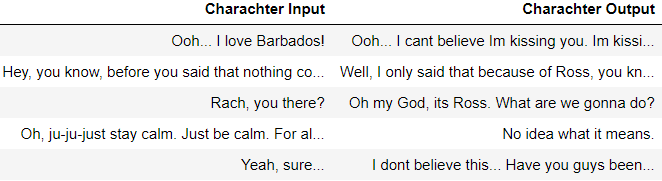
\includegraphics[width=\textwidth]{charachterData.PNG}}
	\end{center}
	\caption{Example of statement response pairs extracted from Friends dataset.}
	\label{fig:friends_data_extracted}
\end{figure}
\begin{figure}[h]
	\begin{center}
		\fbox{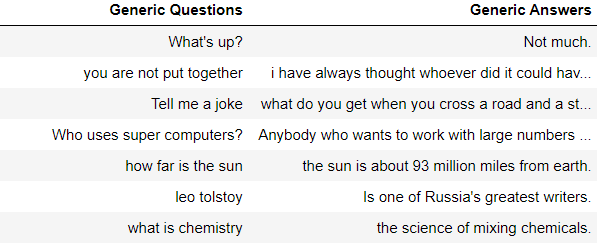
\includegraphics[width=\textwidth]{genericData.PNG}}
	\end{center}
	\caption{Example of statement response pairs extracted from the generic questions and answers dataset.}
	\label{fig:qa_data_extracted}
\end{figure}

To create the personality based chatbot, we first needed a personality to mimic. 
Ideally the personality would be familiar to a large number of people and there would be a large amount of freely available data.
For these reasons we starting looking at characters from popular television shows with multiple seasons.
Moreover, we surmised that the show's writers would have developed a strong and identifiable character personality over the span of several seasons.
We expceted such a personality to be much easier to mimic.
%This gives each character a distinct personality that could be mimicked in a chatbot. 
We also considered movie characters but ultimately, the data available for a movie character was sufficiently smaller than that of a television show character.
%TV show transcripts also offer a larger dataset.

For this project, Friends was chosen as the television show and Joey Tribbiani was chosen as the character. 
We choose Friends because the data was available, the show is popular and it has many seasons.
Joey was chosen to mimic specifically because as has a very distinctive personality in the show. 
For those not familiar the show, Joey can be described as naive, sarcastic, loving, misogynistic, promiscuous and loud.

The raw data set was retrieved from: (https://fangj.github.io/friends/). 
The scrips were split up by episodes with each episode having an associated comma-separated values (CSV) file which held its script.
Each script indicated the character speaking and the dialogue they spoke along with scene discriptions and stage directions (See Figure \ref{fig:friends_data}).
Each script was parsed to extract \emph{statement response pairs} from each scene (See Figure \ref{fig:friends_data_extracted}).
A statement response pair is two dialogues from the script made by two different characters (\emph{stater} and \emph{respondent})the second (\emph{response}) immediately following the first (\emph{statement}).
We then collected all pairs where Joey was the respondent.
We called this the Joey dataset.

%This was done using a python script that pulls keeps track of the previous character that was speaking.
 %If the current character speaking is found to be Joey, the previous character's dialogue is saved as input and the current character's (Joey's) %dialogue is saved as output. 
 %If the current character speaking is not joey the previous character becomes the current character and the algorithm moves on to the next dialogue. This is run across all episode scripts to extract training data. This extraction resulted in around 7000 training data points.

As a prerequisite to training a model to mimic Joey's personality was training a model to sound human in general.
%In additional to having Joey like personalities, we wanted our chatbot to in general respond like a human. 
To this end we wanted to pretrain both our models on an additional dataset of general question and answer pairs. 
Ideally this would help both models to form more proper English sentence and respond appropriately to questions made by the stater.
%The goal of introducing this data set was to help the model understand generic a question answering format. 
Around 500 generic data points were used for training (See Figure \ref{fig:qa_data_extracted}).
We called this the generic question and answer dataset.



%
We randomly selected 20 percent of each dataset to be used as testing data and used the remaining data as training data.
After training and testing our models we realized that there were a few things we could have done to significantly improve our overall experiment. 
We discuss in a later section about what impacts we think the lack of these actions had on our final results.

One key issue with your Joey dataset
In the data extraction process outlined above, we describe collecting using the previous dialogue to any Joey dialogue as a statement.
However, it is easy to see that this is not always ideal.
Indeed, as a result of this, every time a person spoke, regardless of weather Joey heard it or not, Joey's dialogue was considered a response.
Consider the case that Joey enters a scene halfway through and says "hello everyone", this will be recoreded as a response to anything said before his entrance.
%f Monica says something unrelated across the room and Joey responds to something on the television, it is still considered an input output pair. 
Eliminating this problem by implementing a better extraction algorithm could lead to a better dataset and thus better results.

%Another way to augment the data set would be to increase the amount of generic data the model is trained on. 
Another concern is that our generic question and answer dataset was too small and not as generic as desired.
Indeed, more data is always nice but also finding a corpus that had a lot more examples of normal human communication would be ideal.
We believe this process of pretraining on some larger generic dataset would help give each model a better understanding of English.